\chapter{Learning About Oneself}

This chapter follows J. Krishnamurti's first San Diego public talk of April 1970 as an inquiry into action, observation, and learning. There is no blackboard mathematics in the surviving visual material for this lecture, so the displayed formulas below are not recovered equations; they are compact editorial notation for the lecture's conceptual structure. They should be read as a disciplined map of the spoken inquiry, not as a formal psychological theory.

\section{The World As Contradiction}

Krishnamurti begins with the broadest possible field. Wherever one goes, he says, one finds more or less the same human problems: confusion, misery, sorrow, division, conflict, and war. The point is not sociological survey for its own sake. The world is introduced as a field of contradiction so that the question of action can arise with full pressure.

A useful shorthand for the opening movement is
\begin{equation}
\text{division}
\;\longrightarrow\;
\text{contradiction}
\;\longrightarrow\;
\text{conflict}
\;\longrightarrow\;
\text{violence}
\;\longrightarrow\;
\text{sorrow}.
\end{equation}
This is not a theorem. It is the order in which the talk gathers force. National, linguistic, religious, professional, and inward divisions are not treated as separate topics. They are examples of one broken movement.

The same structure appears outwardly and inwardly. The world is divided into nations, sects, professions, ideologies, and rival claims to truth. The person is divided by belief, fear, ambition, anger, comparison, and contradiction. The lecture will not allow these two fields to remain separate for long.

\section{What Is One To Do?}

Seeing this disorder, the question arises: what is one to do? Krishnamurti does not answer at once. He first tests the common answers: left, center, right, ideology, belief, authoritarian dictum, guru, teacher, priest, organized religion, personal inclination, experience, knowledge, confidence, and self-reliance.

The structure of the difficulty is that these alternatives may all belong to the same fragmented field. We may write the first test as
\begin{equation}
\text{programmatic action}
=
\{\text{politics},\text{belief},\text{authority},\text{inclination},\text{experience}\}.
\end{equation}
The notation is deliberately crude. It records the range of offered answers, not a classification system. The important point is that each term can become a fragment claiming authority over life.

\subsection{Question \& Answer}

\paragraph{Question.}
If the world is contradictory, should one follow a political direction, a religious authority, a teacher, a personal tendency, or one's own accumulated experience?

\paragraph{Answer.}
Krishnamurti does not choose one of these. He changes the question. The issue is whether there can be an action that is not born from contradiction and therefore does not produce further sorrow. The inquiry becomes
\begin{equation}
\text{world disorder}
\;\longrightarrow\;
\text{what is one to do?}
\;\longrightarrow\;
\text{whole action}.
\end{equation}

Whole action is introduced negatively before it is described positively. It is not dictated by authority. It is not imitation. It is not dependency. It is not a theory. It is not a philosophical concept. It must be an actual way of living.

\begin{figure}
\centering
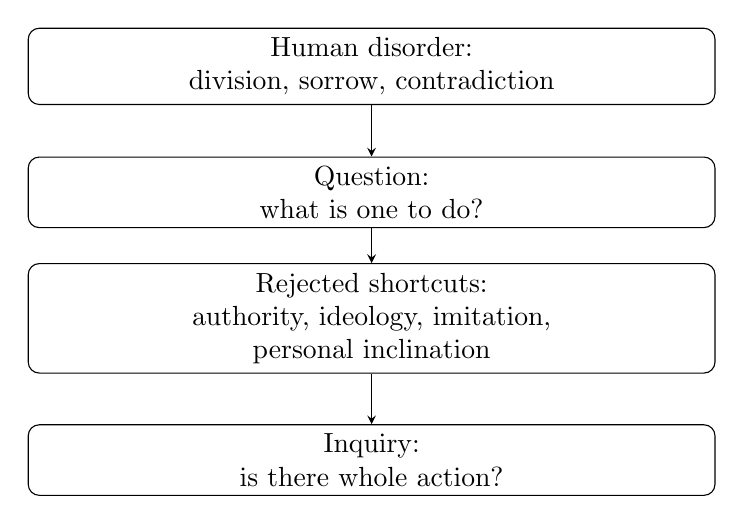
\begin{tikzpicture}[>=stealth]
\node[draw, rounded corners, text width=.70\linewidth, align=center] (a) at (0,0) {Human disorder:\\division, sorrow, contradiction};
\node[draw, rounded corners, text width=.70\linewidth, align=center] (b) at (0,-1.6) {Question:\\what is one to do?};
\node[draw, rounded corners, text width=.70\linewidth, align=center] (c) at (0,-3.2) {Rejected shortcuts:\\authority, ideology, imitation,\\personal inclination};
\node[draw, rounded corners, text width=.70\linewidth, align=center] (d) at (0,-5.0) {Inquiry:\\is there whole action?};
\draw[->] (a) -- (b);
\draw[->] (b) -- (c);
\draw[->] (c) -- (d);
\end{tikzpicture}
\end{figure}

\section{Whole Action And The Speaker As Mirror}

The word ``religion'' is then used in a very specific way. It does not mean belief in God, no-God, or a conceptual system. It means a way of life in which action is whole, complete, and not contradictory. The talk therefore turns from outer programs to the quality of daily living.

We can state the contrast as follows:
\begin{equation}
\text{fragmentary action}
\neq
\text{whole action}.
\end{equation}
Fragmentary action proceeds from division, authority, image, or accumulated knowledge. Whole action is not an occasional response in crisis; it has to concern daily life, every minute, in relationship, speech, thought, and conduct.

At this point Krishnamurti pauses to establish the relation between the speaker and the listener. He is not teaching in the ordinary informational sense. One can teach mathematics or scientific information, but here there is no teacher handing over doctrine. The speaker's words are to be used as a mirror.

\begin{equation}
\text{speaker's words}
\;\longrightarrow\;
\text{listener's reactions}
\;\longrightarrow\;
\text{observation of oneself}.
\end{equation}

This is an important pedagogical move. The listener is not asked to accept a conclusion. The listener is asked to watch reactions, responses, and conditioning as they arise while listening. Communication, in this sense, means sharing, understanding, and working together.

\begin{table}
\centering
\begin{tabular}{p{.42\linewidth}p{.42\linewidth}}
\textbf{Information-learning} & \textbf{Self-learning} \\
Mathematics or scientific information may be taught. & No one can hand over self-understanding. \\
The teacher gives content. & The speaker functions as a mirror. \\
Knowledge is accumulated. & Reaction is observed as it arises. \\
\end{tabular}
\end{table}

\section{The World Is You}

Having made the listener responsible for observation, Krishnamurti returns to the public question. What is one to do about society? The answer changes because the boundary between society and oneself is questioned. Greed, anger, ambition, competition, violence, prejudice, and division are not merely outside. They are inward facts.

The pivot may be written compactly as
\begin{equation}
\text{world} = \text{oneself}
\quad\Longrightarrow\quad
\text{responsibility} = \text{understanding oneself}.
\end{equation}
Again, this is not a metaphysical identity. It is a shorthand for the lecture's claim that the disorder we call society is not separate from the disorder of the human being who has made it.

\subsection{Question \& Answer}

\paragraph{Question.}
If the world is violent and confused, should one ask which party, movement, group, or reform to join?

\paragraph{Answer.}
That question assumes the world is outside oneself. When one sees that one's own greed, ambition, anger, competition, and prejudice are part of the world, the question has a different meaning. Responsibility is no longer primarily the choice of an outer label. It becomes the complete understanding of oneself.

This is the lecture's decisive turn. ``What shall I do?'' becomes ``How shall I observe?''

\section{How To Observe}

The central refrain now appears: how do you observe? Krishnamurti first removes labels. American, Indian, British, religious, ideological, and social labels do not touch the ordinary human being underneath. Then he uses the word ``individual'' in its literal force: indivisible. In that sense, the contradictory human being is not yet an individual.

We can mark the distinction as
\begin{align}
\text{individual} &:= \text{undivided human being},\\
\text{ordinary self} &:= \text{fragmented, contradictory movement}.
\end{align}

The question becomes sharper. If the self is fragmented, can one fragment observe the rest? If one fragment becomes the censor, examiner, analyser, or observer, what gives that fragment authority?

\begin{figure}
\centering
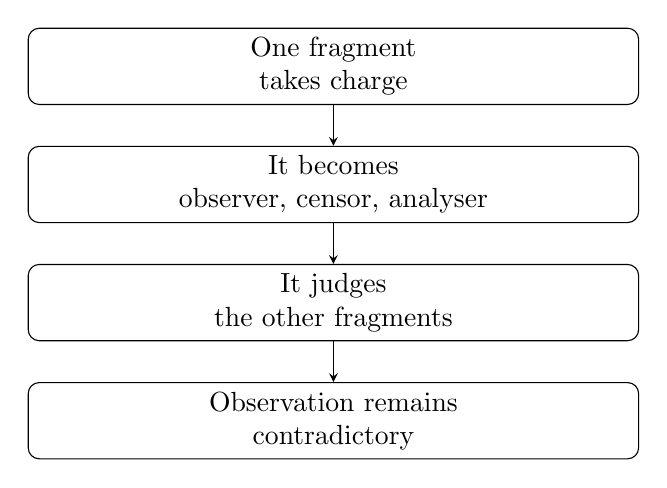
\begin{tikzpicture}[>=stealth]
\node[draw, rounded corners, text width=.62\linewidth, align=center] (f1) at (0,0) {One fragment\\takes charge};
\node[draw, rounded corners, text width=.62\linewidth, align=center] (f2) at (0,-1.5) {It becomes\\observer, censor, analyser};
\node[draw, rounded corners, text width=.62\linewidth, align=center] (f3) at (0,-3.0) {It judges\\the other fragments};
\node[draw, rounded corners, text width=.62\linewidth, align=center] (f4) at (0,-4.5) {Observation remains\\contradictory};
\draw[->] (f1) -- (f2);
\draw[->] (f2) -- (f3);
\draw[->] (f3) -- (f4);
\end{tikzpicture}
\end{figure}

This is why the inquiry cannot stop with self-analysis. Whether one is analysed by a professional or analyses oneself, the same pattern may continue if one fragment claims authority over the rest. The observer is not yet free of the field it observes.

\begin{proposition}
If the observer is itself a fragment, then observation by that observer cannot end fragmentation.
\end{proposition}

\begin{proof}
The observer is one part of the divided field. When that part claims authority over the other parts, division has not ended; it has merely taken a hierarchical form. The observer may condemn, justify, approve, store up, or attempt control, but those movements are themselves fragmentary. Therefore the observation remains within contradiction.
\end{proof}

\section{The Observer, The Image, And Violence}

Krishnamurti next asks whether we observe through an image. We look at a tree through knowledge of the tree. We look at wife, husband, friend, opponent, Catholic, Protestant, communist, or bourgeois through images accumulated over years or days. The image stands between observer and observed.

The sequence is
\begin{equation}
\text{knowledge}
\;\longrightarrow\;
\text{image}
\;\longrightarrow\;
\text{observer}
\;\longrightarrow\;
\text{separation}.
\end{equation}

The image becomes the observer. That is the crucial movement. The observer is not a neutral witness outside conditioning. It is built from memory, judgement, naming, hurt, flattery, insult, belief, and fear.

The lecture tests this not as an abstraction but through violence. Suppose I am violent: angry, jealous, brutal, ambitious, comparing myself with another. If I then say, ``I must get rid of violence,'' who is the ``I'' that says this? Is it separate from violence, or is it another form of the same movement?

\subsection{Question \& Answer}

\paragraph{Question.}
Is the observer different from violence?

\paragraph{Answer.}
Krishnamurti's answer is that the separation is one of the tricks of thought. The observer who condemns violence, justifies violence, or tries to escape violence is not outside violence. In this local and precise sense,
\begin{equation}
\text{observer} = \text{observed}.
\end{equation}
This is not a mathematical identity and not a general metaphysical slogan. It means that the observer looking at violence is part of the same movement as violence.

The contrary assumption may be written
\begin{equation}
\text{observer} \neq \text{observed}
\quad\Longrightarrow\quad
\text{division}
\quad\Longrightarrow\quad
\text{conflict}.
\end{equation}
So long as there is a division between observer and observed, conflict continues. When the observer sees that it is not separate from the observed, the structure of condemnation and escape changes.

\begin{figure}
\centering
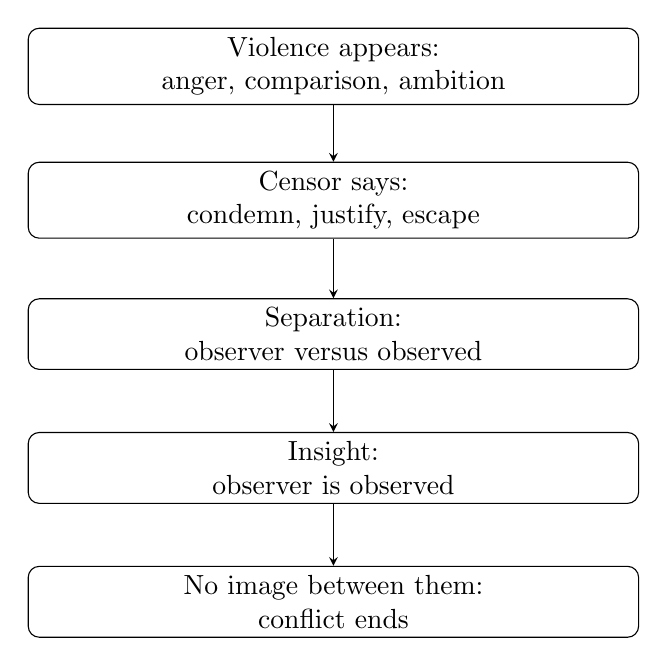
\begin{tikzpicture}[>=stealth]
\node[draw, rounded corners, text width=.62\linewidth, align=center] (a) at (0,0) {Violence appears:\\anger, comparison, ambition};
\node[draw, rounded corners, text width=.62\linewidth, align=center] (b) at (0,-1.7) {Censor says:\\condemn, justify, escape};
\node[draw, rounded corners, text width=.62\linewidth, align=center] (c) at (0,-3.4) {Separation:\\observer versus observed};
\node[draw, rounded corners, text width=.62\linewidth, align=center] (d) at (0,-5.1) {Insight:\\observer is observed};
\node[draw, rounded corners, text width=.62\linewidth, align=center] (e) at (0,-6.8) {No image between them:\\conflict ends};
\draw[->] (a) -- (b);
\draw[->] (b) -- (c);
\draw[->] (c) -- (d);
\draw[->] (d) -- (e);
\end{tikzpicture}
\end{figure}

Around this point the transcript is partly damaged, but the surrounding movement is clear. Identification is also part of separation: the mind separates itself as censor and then tries to identify with what it calls beautiful or noble. Where there is no image between observer and observed, Krishnamurti says, conflict comes to an end. He calls this real meditation, not a trick.

\section{Learning Without Accumulation}

The last difficulty is subtler. One observes oneself and learns something. Then, the next minute, one looks again through what one has learned. Has learning continued, or has yesterday's observation become another form of knowledge?

We can model this carefully as a warning, not as a doctrine. Let $I_n$ denote the image or accumulated residue through which one looks at moment $n$. A usual movement of accumulation is
\begin{equation}
I_{n+1}=I_n\cup\{\text{insult},\text{flattery},\text{judgement},\text{previous observation}\}.
\end{equation}
Then the next act of seeing is filtered through $I_{n+1}$:
\begin{equation}
\text{seeing}_{n+1}
=
\text{observation through } I_{n+1}.
\end{equation}
Krishnamurti's difficulty is that such accumulated knowledge prevents fresh perception. The accumulation itself becomes the observer, the censor, the conditioned entity.

\paragraph{Worked example: flattery and insult.}
Suppose someone says, ``How intelligent you are,'' or ``How stupid you are.'' If the words are accumulated, the update is
\begin{align}
I_{n+1}
&= I_n \cup \{\text{flattery}\}
&&\Longrightarrow\quad \text{the speaker becomes friend},\\
I_{n+1}
&= I_n \cup \{\text{insult}\}
&&\Longrightarrow\quad \text{the speaker becomes enemy}.
\end{align}
In either case, listening has created an image. The image separates. From then on one no longer listens directly; one listens through the stored picture.

The alternative is not suppression and not a cultivated technique. It is to listen without accumulating the insult or the flattery. The same structure applies to anger. If one is not aware at the moment of anger, the image is already forming; the observer as censor has already taken its place.

\begin{definition}
Observation without accumulation means looking or listening without carrying forward insult, flattery, naming, previous conclusion, or self-image as the basis for the next perception.
\end{definition}

The lecture closes this movement with simple examples: cloud, hills, light on water. To observe without naming is to see how naming, knowledge, and experience can prevent the mind from observing totally. When the mind looks without the observer, the fragments come to an end in oneself. This, Krishnamurti says, cannot be taught by another.

\section{Summary}

The chapter's logical movement is compact, but the lecture unfolds it slowly. Human life is divided, and division expresses itself as contradiction, conflict, violence, and sorrow. The question ``what is one to do?'' cannot be answered by another fragment: not by ideology, belief, authority, personal inclination, or accumulated experience.

The inquiry therefore turns to whole action, and then to observation. The speaker is not a teacher in the ordinary sense but a mirror. The world is not merely outside oneself; the world and the self share the same structure of greed, anger, ambition, competition, violence, prejudice, and division.

The central problem becomes: how do we observe? If one fragment observes the rest, the observer is still part of fragmentation. If we observe through image, knowledge, naming, flattery, insult, or accumulated experience, the image becomes the observer and separation continues. In the decisive formulation of the lecture, the observer is the observed. To see this directly, without making it a slogan or a method, is the act of learning.